\documentclass[11pt]{article}
\usepackage{parskip,times, hyperref, cite, url, graphicx, float}
\usepackage[margin=1.5in]{geometry}

\begin{document}

\vspace{-2em}
\centerline{\large \emph{L46 Project}}
\vspace{2em}
\centerline{\Large \emph{Exploring Quantisation In FPGA-Accelerated Binarized Neural Networks}}
\vspace{2em}
\centerline{\large Alex Chau (\emph{ac2822}), Churchill College}
\section{Introduction}
The rapid advancement of machine learning has driven an increasing demand for efficient hardware acceleration of neural networks. 
While general-purpose processors such as CPUs and GPUs have traditionally been used for this purpose, significant performance and energy efficiency gains have emerged from the use of specialised hardware accelerators.
In particular, field-programmable gate arrays (FPGAs) have gained attention due to their ability to provide flexible, fine-grained parallelism and custom dataflow architectures tailored to specific workloads.

A key technique enabling these improvements is quantisation, which reduces the numerical precision of neural network parameters and activations. 
By representing values with fewer bits, ranging from reduced fixed-point precision to fully binarized representations, quantisation significantly lowers memory usage and computational complexity. 
This, in turn, allows for faster inference, reduced power consumption, and more efficient utilisation of hardware resources. 
In extreme cases such as binarized neural networks (BNNs), arithmetic operations can be simplified to bitwise operations, making them especially well-suited for FPGA implementations.

Much of the recent progress in the AI hardware acceleration space can be attributed to the combination of increased hardware specialisation and aggressive quantisation strategies. 
Specialised architectures are able to exploit the reduced precision of quantised models to maximise parallelism and throughput, achieving performance levels that would be difficult to attain with conventional high precision designs.

This project explores the role of quantisation in FPGA-accelerated neural networks, with a particular focus on binarized neural networks.
Using the FINN framework, quantized models are mapped to dataflow-style hardware architectures on an FPGA platform. 
The study investigates how neural networks trained in Brevitas are mapped to FPGA-accelerated neural networks and how different levels of quantisation that impact performance, as well as how these effects interact with architectural parallelism. 
Through these experiments, the project aims to provide insight into the trade-offs between accuracy, resource utilisation, and performance in quantised neural network deployment on reconfigurable hardware.
\section{Experiment 1: Analysis of the PyTorch to FPGA transformation pipeline for Quantized Neural Networks}
\subsection{System Setup}
To evaluate quantized neural network acceleration on FPGA hardware, the FINN framework was deployed on a Diligent Arty-Z7-20 development board.
FINN is an open-source framework developed by Xilinx/AMD that enables deployment of quantized neural networkks (QNNs) on FPGA platforms through automated hardware generation and compilation.
\subsubsection{Hardware Platform}
The target platform used in this project is the Arty-Z7-20 development board, this board includes an Artix-7 FPGA as the programmable logic (PL) and an ARM Cortex-A9 processor in the form of a Zynq-7000 SOC as the programmable system (PL).
\subsubsection{Software Environment}
\begin{itemize}
    \item{PYNQ - A pre-built Linux image for Zynq SOCs (which interfaces with PL using Python) was flashed onto a microSD card and inserted onto the board.} 
        \begin{itemize}
            \item{There are a small number of pre-built images which AMD maintains, the Arty-Z7-20 isn't one of these boards. 
                Luckily, one of the supported boards (Pynq-Z1), happens to have the exact same specs and (almost the same) pinouts as the Arty-Z7-20, making PYNQ images built for the Pynq-Z1 compatible with the Z7-20, we use the PYNQ v3.0.1 image in this work}
        \end{itemize}
    \item{FINN - A compiler which maps Quantized Neural Networks (QNNs) trained in Brevitas to dataflow-style FPGA architectures \cite{umurogluFINNFrameworkFast2017}.}
    \item{Xilinx Design Suite 2022.2}
\end{itemize}
\begin{figure}[H]
    \centering
    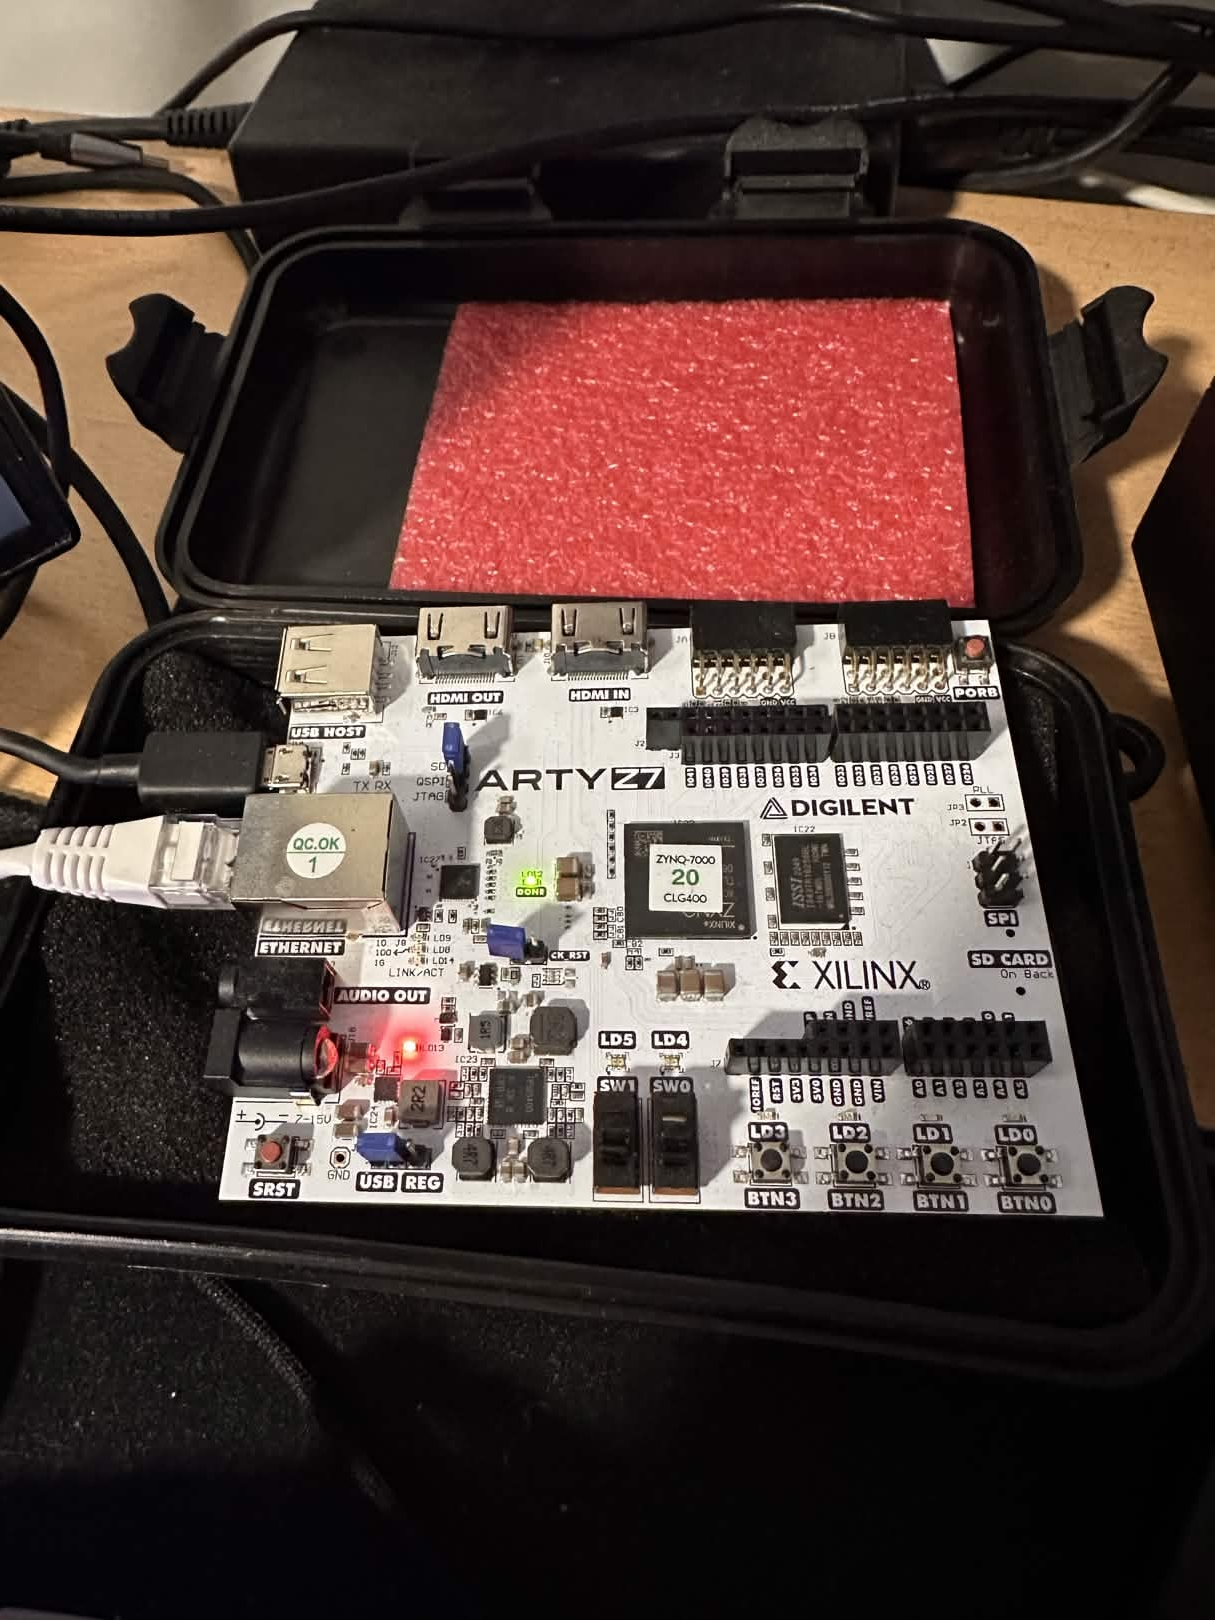
\includegraphics[width=1\linewidth]{Images/artyBoard.jpg}
    \caption{Image of the Arty-Z7-20}
    \label{fig:devBoard}
\end{figure}
The rest of this subsection will detail the steps to replicate the environment for training quantized neural networks using Brevitas and converting it to a FPGA-deployable bitstream using the FINN compiler.
\subsubsection{Ubuntu 24.04}
Ubuntu 24.04 was selected as the development OS for a couple of reasons: The FINN compiler has dependencies better suited to UNIX-like operating systems, a NVIDIA GPU (RTX 3090) was the GPU available for training quantized neural networks, and Vivado tooling is hard to setup with FINN in a non-Unix environment.
Ubuntu was installed following the interactive installer, one-thing to note is that the Vivado install uses a large amount of data in the /tmp directory. Some Ubuntu install guides recommend allocating a separate 20-30GB partition purely for /tmp, we recommended allocating only a single root partition for the install so that tmp doesn't run out of memory during the Vivado Design Suite Installation, as it uses over 80GB of /tmp memory.
\subsubsection{Xilinx Design Suite 2022.2}
The FINN compiler currently only supports Vivado Design Suite 2022.2, this is slightly troublesome as the newest version of Ubuntu this Vivado version supports is Ubuntu 22.04.
We (libtinfocurses stupid thing)
\subsubsection{FINN}
in here mention about how FINN has a version of Brevitas which has an outdated train.py script, 
\subsubsection{PYNQ/Development Board}
Say some stuff about having to move the jumpers on the board, flashing the PYNQ image, setting up internet connection
\subsection{Training a BNN using Brevitas}
\subsection{Preparing a trained Brevitas network for hardware synthesis}
\subsection{Evaluating the BNN compared to running on a GPU // Something like this}
\section{Experiment 2: Impact of quantisation on neural network FPGA performance}
\section{Experiment 3: Investigating parallelism in FPGA QNN performance}
Basically see if parallelism with certain quantisation sizes has some impact.
Use minimal, small, and the w1a1 things in hardware
\newpage
\bibliography{library}{}
\bibliographystyle{plainurl}
\end{document}
